\title[Distribuované reprezentace]{Distribuované reprezentace slov}
\subtitle{Odhady pravděpodobnostní funkce, neuronové sítě a~faktorizace}
\author[V.\,Novotný]{Vítek Novotný \\ witiko@mail.muni.cz}
\institute[FI MU]{Fakulta Informatiky, Masarykova Univerzita}
\date{18.\ října 2018}
\subject{Distribuované reprezentace polysémních slov}
\keywords{vector space model, neural networks, word embeddings}

\begin{frame}[plain]%
\maketitle

\mode
<presentation>

\begin{tikzpicture}[overlay,remember picture]
    \node[anchor=south east, xshift=-20pt, yshift=60pt] at (current page.south east) {
      \raisebox{-30pt}{
\includegraphics[width=90pt]{figs/magnifyingglass}}%
      \hspace{-99pt}\huge$\hat P(\text{\textbf{word}}\mid\text{context})$
    };
\end{tikzpicture}

\mode
<all>

\end{frame}


\mode
<presentation>

\begin{frame}{Obsah}
\tableofcontents
\end{frame}

\mode
<article>

\tableofcontents

\mode
<all>

\section{Úvod}

\begin{frame}{Úvod}
Cílem semináře je shrnout historii a~navazující výzkum související
s~distribuovanými reprezentacemi slov, které popisují~\textcite{mikolov13a}.
Diskuze by se měla zaobírat řešením problému víceznačnosti v~distribuovaných
reprezentacích.
\end{frame}

\section{Odhady pravděpodobnostní funkce}
\subsection{Naivní jazykové modely}

\begin{frame}{Naivní jazykové modely}
Z~hlediska vyhledávání je cílem statistických \emph{jazykových
modelů}\index{jazykový model} především bodový odhad $\hat P$ pravděpodobnostní
funkce $P(d)$, kde $d$ je dokument. Toto umožňuje dokumenty generovat a~řadit
podle $\hat P$.
\autocites[kap.~12]{manning08}{ponte98}{hiemstra98}{berger99}{miller99}

\pause

\begin{itemize}[<+->]
\item Naivní model předpokládá, že dokument $d$ je náhodný vektor obsahující
  stejně rozdělené \emph{nezávislé} náhodné veličiny, které generují
  \emph{termy}\index{term} (fráze, slova, lemmata, $n$-gramy, atp.) $w_t$.
  V~tomto modelu
\mode
<presentation>
  $P(d) = P(w_1, \ldots, w_{|d|}) = P(w_1^{|d|}) = \prod_{t=1}^{|d|} P(w_t)$.
\mode
<article>
  platí
  $$P(d) = P(w_1, \ldots, w_{|d|}) = P(w_1^{|d|}) = \prod_{t=1}^{|d|} P(w_t).$$
\mode
<all>
\item Střízlivější model bere v~potaz, že bezprostředně následující termy nelze
  považovat za nezávislé. Namísto toho se zavádí \emph{kontext}\index{kontext
  termu} délky $n$ a~předpokládá se, že $P(w_t\mid w_1^{t-1})\approx
  P(w_t\mid w_{t-n+1}^{t-1})$. V~tomto modelu $P(d) = P(w_1^{|d|}) =
  \prod_{t=1}^{|d|} P(w_t\mid w_1^{t-1})\approx \prod_{t=1}^{|d|} P(w_t\mid
  w_{t-n+1}^{t-1})$.
\end{itemize}
\end{frame}

\begin{frame}{State-of-the-art před distribuovanými reprezentacemi slov}
State-of-the-art jazykové modely z~80.\ let vychází ze střízlivějšího
modelu a~řeší problémy spojené s~odhadem $P(w_t\mid w_1^{t-1})$.

\pause

\begin{itemize}[<+->]
\item Při \emph{maximálně věrohodném}\index{odhad!maximálně věrohodný} (MLE)
  odhadu
\mode
<presentation>
  $\hat P(w_t\mid w_{t-n+1}^{t-1}) = \frac{\text{Počet
  výskytů }w_{t-n+1}^{t}}{\text{Počet výskytů }w_{t-n+1}^{t-1}}$.
\mode
<article>
  platí
  $$\hat P(w_t\mid w_{t-n+1}^{t-1}) = \frac{\text{Počet
  výskytů }w_{t-n+1}^{t}}{\text{Počet výskytů }w_{t-n+1}^{t-1}}.$$
\mode
<all>
  Zároveň ale
  s~rostoucí délkou kontextu $n$ roste počet posloupností $w_{t-n+1}^{t-1}$,
  které se v~trénovacích datech nevyskytnou. Následně $\hat P(w_t\mid
  w_{t-n+1}^{t-1}) = 0$ a~tedy $\hat P(d) = 0$.
\begin{itemize}[<+->]
\item Inženýrským řešením je \emph{vychýlený}, \emph{asymptoticky
  konzistentní} odhad, který předpokládá, že se každá posloupnost vyskytla
o~jednou víckrát.~\autocites{lidstone20}\index{odhad!asymptoticky
  konzistentní}\index{odhad!vychýlený}
\item \textcite{jelinek80} odhadují $P(w_t\mid w_1^{t-1})$ iterpolací --
  lineární funkcí MLE odhadů $P(w_t\mid w_{t-n+1}^{t-1})$ pro různé délky
  kontextu $n$. \textcite{katz87} využívá \emph{Turingovu
  metodu}\index{Turingova metoda}~\autocites{good53, nadas85} pro odhad
  parametrů lineární funkce.
\end{itemize}
\item S~rostoucí délkou kontextu $n$ exponenciálně roste velikost tabulky
  s~počty výskytů.
\begin{itemize}[<+->]
\item Uspokojivě vyřešeno až distribuovanými reprezentacemi slov.
\end{itemize}
\end{itemize}
\end{frame}

\subsection{Distribuované reprezentace slov}

\begin{frame}<1-2>[label=bengio03_mikolov13a]{Distribuované reprezentace slov}
\emph{Distribuovaná reprezentace slov}\index{distribuovaná reprezentace slov}
nahrazuje tabulku s~počty výskytů za slovní vektory.
\looseness=-1

\pause

\begin{itemize}[<+->]
\item \textcite{bengio03} navrhují síť, která hledá funkci
  $f, f(w_t, w_{t-n+1}^{t-1}) = P(w_t\mid w_1^{t-1})$.
\only<1-5>{\begin{itemize}[<+->]
\item Výstupní vrstva $\mathbf{y}$ je transformována \emph{softmax
  funkcí $\sigma$}\index{softmax},
  $\sigma(\mathbf{y})_i = \frac{e^{y_i}}{\sum_j e^{y_j}},$ pro kterou platí
  $\sigma(\mathbf{y})_i \in[0, 1], \sum_i\sigma(\mathbf{y})_i = 1$. Toto
  zajistí zachování axiomů pravděpodobnostní funkce.
\item Nejlepších výsledků autoři dosahují s~odhadem $P(w_t\mid w_1^{t-1})$, který
  je lineární funkcí interpolovaného odhadu $P(w_t\mid
  w_1^t)$ \autocites{jelinek80} a~$f$.
\item \emph{Zpětná propagace}\index{zpětná propagace} maximalizuje
  \emph{věrohodnost}\index{věrohodnost modelu}
  $\mathcal{L}(\theta\mid d) = \prod_{i=1}^{|d|} f(w_t,$
  $w_{t-n+1}^{t-1}\mid\theta)$
  plus $R(\theta),$ kde $\theta$ je matice $C$
  a~váhy sítě a~$R(\theta)$ je regularizační faktor penalizující velké hodnoty
  $\theta$.
\end{itemize}}
\item \textcite{mikolov13a} aktualizují síť podle~\textcite[sekce 5]{bengio03}.
  \looseness=-1
\only<7-9>{\begin{itemize}
\item<7-9> Zahazuje se informace o~pořadí slov v~kontextu.
\item<7-9> „\foreignlanguage{english}{In the neural network […] the distributed word features are used only
  for the ‘input’ words and not for the ‘output’ word […]
  similarities between output words are not exploited.}“ Nová architektura
  obsahuje matice $\mathbf W, \mathbf W'$ pro vstupní a~výstupní termy.
\item<8-9> „\foreignlanguage{english}{Representing the conditional probability with a~tree
  structure […] has the potential to reduce computation time by a~factor
  $|V|\log|V|$.}“ \textcite{mikolov13a} využívají \emph{hierarchální
  softmax}\index{softmax!hierarchální}~\autocites{mikolov11}{mnih09}{morin05}[sekce 3.1]{rong14}.
\item<9-9> „\foreignlanguage{english}{Propagating gradients only from a~subset of the output words.}“
  \textcite{mikolov13c} aktualizují výstupní vektor pouze trénovaného slova
    a~malého \emph{negativního vzorku}\index{negativní vzorek} dalších slov
    jako alternativu k~hierarchálnímu softmaxu.
\end{itemize}}
\item<10-12> \textcite{mikolov13a} navrhují hledat funkci
  $f', f'(w_t, w_{t-n+1}^{t-1}) = P(w_1^{t-1}\mid w_t)$.
\only<11-12>{\begin{itemize}
\item<11-12> Continuous Bag-of-Words (CBOW) je architektura, která hledá funkci $f$.
  Zpětná propagace maximalizuje věrohodnost
  $\mathcal{L}(\theta\mid w_t) = \prod_{i=1}^{|d|} f(w_t,$
  $w_{t-n+1}^{t-1}\mid\theta),$ kde $\theta$ jsou matice $\mathbf W, \mathbf W'$.
\item<12-12> Skip-gram je architektura, která hledá funkci $f'$.
  Zpětná propagace maximalizuje věrohodnost
  $\mathcal{L'}(\theta\mid w_t) = \prod_{i=1}^{|d|} f'(w_t,$
  $w_{t-n+1}^{t-1}\mid\theta),$ kde $\theta$ jsou matice $\mathbf W, \mathbf W'$.
\end{itemize}}
\end{itemize}
\mode
<presentation>
\vspace{10cm}
\mode
<all>
\end{frame}

\begin{frame}
\begin{figure}[H]
\begin{center}
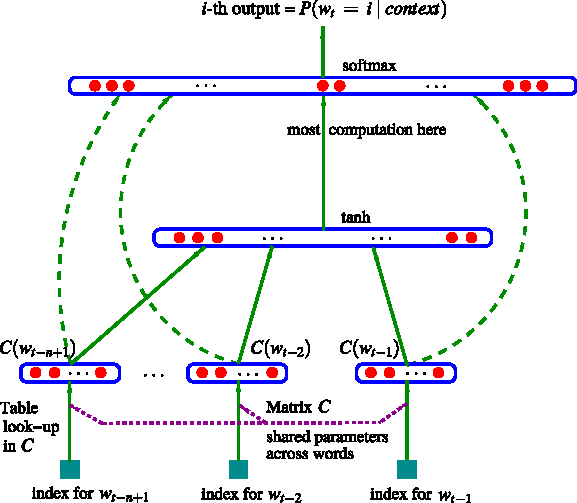
\includegraphics[width=0.5\paperwidth]{figs/bengio03}
\bigskip\par
Zdroj: \textcite{bengio03}
\end{center}
\end{figure}
\end{frame}

\againframe<2-7|handout:0>{bengio03_mikolov13a}

\begin{frame}
\begin{figure}[H]
\begin{center}
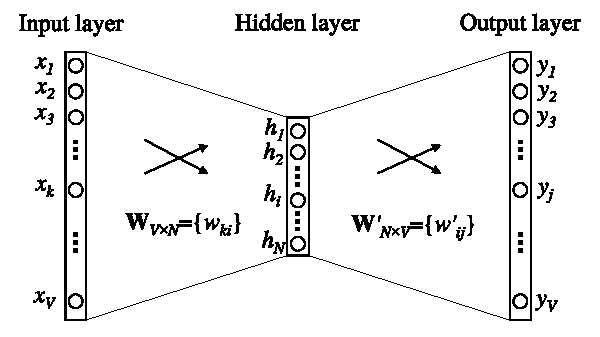
\includegraphics[width=0.5\paperwidth]{figs/rong14_fig1}
\bigskip\par
Zdroj: \textcite[obrázek 1]{rong14}
\end{center}
\end{figure}
\end{frame}

\againframe<7-8|handout:0>{bengio03_mikolov13a}

\begin{frame}
\begin{figure}[H]
\begin{center}

\mode
<presentation>

\includegraphics[width=0.7\paperwidth]{figs/rong15}

\mode
<article>

\includegraphics[width=0.5\paperwidth]{figs/rong15}

\mode
<all>

\bigskip\par
Zdroj: \textcite[strana 34]{rong15a}
\end{center}
\end{figure}
\end{frame}

\againframe<8-11|handout:0>{bengio03_mikolov13a}

\begin{frame}
\begin{figure}[H]
\begin{center}
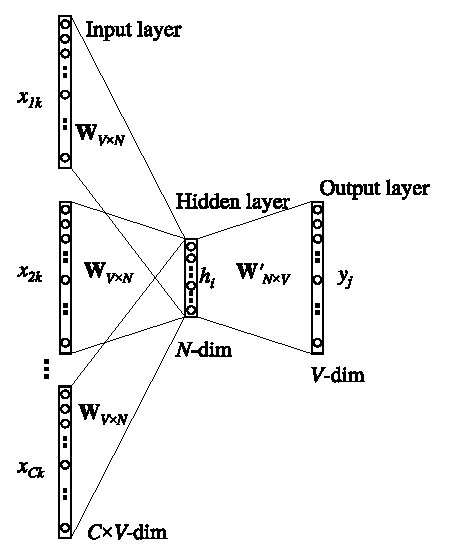
\includegraphics[width=0.3\paperwidth]{figs/rong14_fig2}
\bigskip\par
Zdroj: \textcite[obrázek 2]{rong14}
\end{center}
\end{figure}
\end{frame}

\againframe<11-12|handout:0>{bengio03_mikolov13a}

\begin{frame}
\begin{figure}[H]
\begin{center}
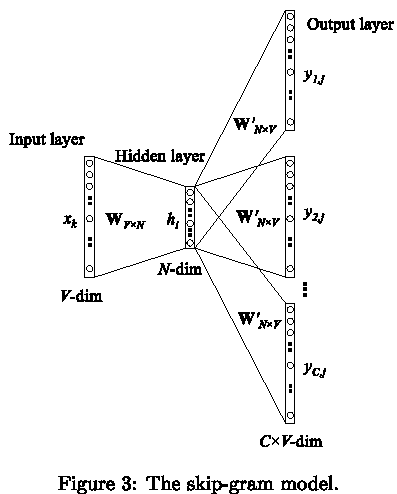
\includegraphics[width=0.3\paperwidth]{figs/rong14_fig3}
\bigskip\par
Zdroj: \textcite[obrázek 3]{rong14}
\end{center}
\end{figure}
\end{frame}

\againframe<12|handout:0>{bengio03_mikolov13a}

\section{Hledání slovních analogií}
\subsection{Neuronové sítě}

\begin{frame}<1-2>[label=word_analogy]{Hledání slovních analogií}
\textcite{mikolov13c} si jako první všímá, že slovní vektory v~rámci
distribuovaných reprezentací lze využít pro hledání analogií mezi termy.
„$\text{King} - \text{Man} + \text{Woman} = \text{Queen}.$“

\pause

\begin{itemize}[<+->]
\item Skip-gram architektura~\autocites{mikolov13a} generuje vektory, které dávají
  lepší výsledky při hledání analogií.
\item \textcite{levy14c} ukazují, že lepší výsledky dává vektorový součin.
	„$\text{King} / \text{Man} \cdot \text{Woman} = \text{Queen}.$“
\item \textcite[strana 40]{rong15a} uvádí další architektury neuronových sítí
	použitelné pro generování vektorů, které lze využít pro hledání analogií.
\end{itemize}
\end{frame}

\begin{frame}
\begin{figure}[H]
\begin{center}

\mode
<presentation>

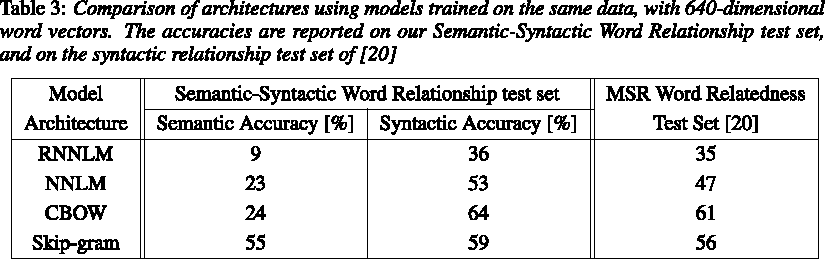
\includegraphics[width=0.8\paperwidth]{figs/mikolov13a_table3}

\mode
<article>

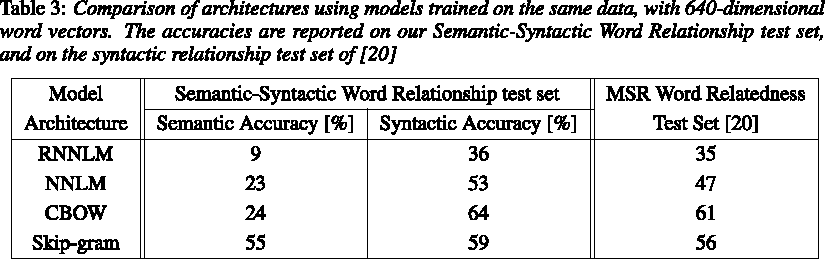
\includegraphics[width=0.6\paperwidth]{figs/mikolov13a_table3}

\mode
<all>

\bigskip\par
Zdroj: \textcite{mikolov13a}
\end{center}
\end{figure}
\end{frame}

\againframe<2-3|handout:0>{word_analogy}

\begin{frame}
\begin{figure}[H]
\begin{center}
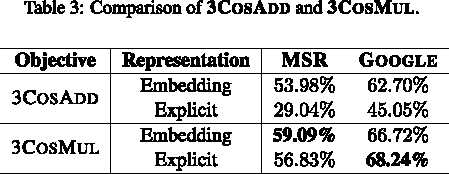
\includegraphics[width=0.4\paperwidth]{figs/levy14c_table3}
\bigskip\par
Zdroj: \textcite{levy14c}
\end{center}
\end{figure}
\end{frame}

\againframe<3-4|handout:0>{word_analogy}

\subsection{Faktorizace matic}

\begin{frame}{Faktorizace matic}
Série článků od Levyho et al. z~let 2014 a~2015 ukazuje, že neuronové sítě pro
hledání distribuovaných reprezentací termů provádí implicitní faktorizaci
\emph{matice souvýskytů}\index{matice souvýskytů} termů.

\pause

\begin{itemize}[<+->]
\item \cite{levy14b} ukazují, že pomocí matice \emph{pointwise mutual
  information}\index{pointwise mutual information} (PMI) mezi termem a~kontexty
  lze získat vektory, které lze využít pro hledání analogií.
\item \cite{levy15} ukazují, že pokud se kontrolují hyperparametry
	související s~neuronovými sítěmi, dávají vektory z~PMI matice při hledání
	analogií srovnatelné výsledky s~neuronovými sítěmi.
\end{itemize}

\pause

\textcite[36 minut a~40 sekund]{rong15b} uvádí, že neuronové sítě jsou stále
výhodnější z~hlediska \emph{prostorové složitosti}\index{prostorová složitost}.
Zatímco faktorizace vyžaduje explicitní reprezentaci PMI matice typu
$|V|\times|V|^n$, kde $V$ je množina termů, neuronová síť s~CBOW nebo Skip-gram
architekturou vyžaduje pouze explicitní reprezentaci dvou matic $\mathbf W,
\mathbf W'$ typu $|V|\cdot m,$ kde $m$ je dimenze slovních vektorů.

\end{frame}

\subsection{Problém polysémie}

\begin{frame}{Problém polysémie}
V~distribuovaných reprezentacích mnohoznačných termů dochází ke~zprůměrování
různých významů termu do jednoho slovního vektoru, což zhoršuje přesnost
modelu.

\pause

\begin{itemize}[<+->]
\item\textcite[sekce 5]{bengio03} uvádí „\foreignlanguage{english}{Polysemous words
are probably not well served by the model presented here, which assigns to each
word a~single point in a~continuous semantic space. We are investigating
extensions of this model in which each word is associated with multiple points
in that space, each associated with the different senses of the word.}“ Na
žádné navazující publikaci řešící \emph{vícevýznamové distribuované
reprezentace}\index{distribuovaná reprezentace slov!vícevýznamová} se však
žádný z~autorů nepodíli.
\item\textcite{li15} navrhují neuronovou síť, která pomocí procesu \emph{Bayesovské
  inference (Chinese restaurant process)}\index{Chinese restaurant process}
  \index{Bayesovská inference} vytváří slovní vektory pro jednotlivé významy termů.
\end{itemize}
\end{frame}

\section{Závěr a~diskuze}

\begin{frame}[plain]
\vfill
\centerline{Děkuji vám za pozornost!}
\vfill\vfill
\end{frame}

\mode
<presentation>

\section{Bibliografie}

\begin{frame}[allowframebreaks]{Bibliografie}
\printbibliography
\end{frame}

\mode
<article>

\printbibliography

\printindex

\mode
<all>
